%----------------------------------------------------------------------------------------
%	PACKAGES AND THEMES
%----------------------------------------------------------------------------------------
\documentclass[aspectratio=169,xcolor=dvipsnames]{beamer}
\usetheme{SimplePlus}

\usepackage[brazilian]{babel}
\usepackage[utf8]{inputenc}
\usepackage{hyperref}
\usepackage{graphicx} % Allows including images
\usepackage{booktabs} % Allows the use of \toprule, \midrule and \bottomrule in tables
% \usepackage[table,dvipsnames]{xcolor}
\usepackage{tikz,tkz-base, tkz-fct,tikz-3dplot,tikz-cd,tkz-tab,tkz-euclide,pgf,pgfplots}
\usepackage{pstricks}
\usepackage{pst-plot}
\usepackage{systeme}
\usepackage{multicol}
\usepackage{lmodern,mathrsfs}
\usepackage{tasks}
\usepackage{float}
\usepackage{array}
\usepackage{multirow}
\usetikzlibrary{matrix} % LATEX and plain TEX

\pgfplotsset{compat=newest}

%----------------------------------------------------------------------------------------
%	TITLE PAGE
%----------------------------------------------------------------------------------------

\title[short title]{Matrizes} % The short title appears at the bottom of every slide, the full title is only on the title page
% \subtitle{Subtitle}

\author[Fernando-Jorge] {Fernando Jorge}

\institute[NTU] % Your institution as it will appear on the bottom of every slide, may be shorthand to save space
{
  Escola Estadual Professor Lima Castro
}
\date{\today} % Date, can be changed to a custom date


%----------------------------------------------------------------------------------------
%	PRESENTATION SLIDES
%----------------------------------------------------------------------------------------

\begin{document}

\begin{frame}
    % Print the title page as the first slide
    \titlepage
\end{frame}

\begin{frame}{Sumário}
    % Throughout your presentation, if you choose to use \section{} and \subsection{} commands, these will automatically be printed on this slide as an overview of your presentation
    \tableofcontents
\end{frame}

%------------------------------------------------
\section{Introdução}
%------------------------------------------------

\begin{frame}{Problema 1 - O muro das subtrações}
    Cada um dos tijolos do muro desenhado abaixo repousa sobre outros dois tijolos.
    O valor inscrito em cada um deles representa a diferença entre os números
    inscritos nos tijolos sobre os quais está apoiado. Complete os números
    que faltam, sabendo que na fila de baixo os dígitos de \textbf{0} a \textbf{9}
    só aparecem uma vez.
  \begin{figure}[htb!]
    \centering
    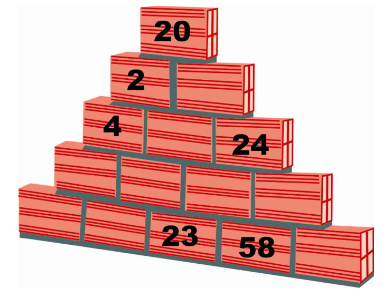
\includegraphics[width=.4\linewidth]{images/muro.png}
  \end{figure}
\end{frame}

%------------------------------------------------

\begin{frame}{Problema 2 - Somas ocultas}
    Preencha as casas vazias deste esquema com números de \textbf{11} a \textbf{35},
    colocando os ímpares nos círculos e os pares nos triângulos. Regras: a soma
    de uma linha qualquer (como de \textbf{A} a \textbf{K}) sempre deve dar \textbf{115}.
    Na casa \textbf{A} deve entrar o maior número ímpar e na \textbf{D}, o menor par.
    \textbf{K} é a soma de \textbf{D} com \textbf{2} e \textbf{V} é igual a
    \textbf{J} mais \textbf{6}.

  \begin{figure}[htb!]
    \centering
    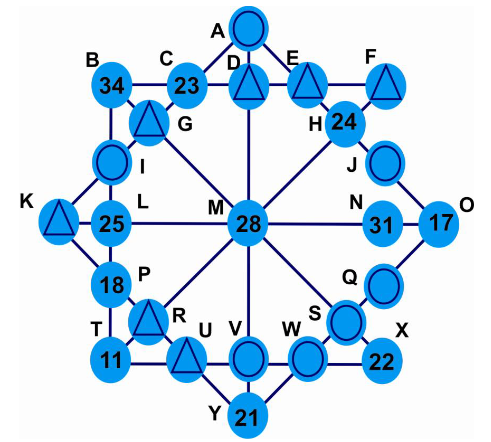
\includegraphics[width=.4\linewidth]{images/soma-oculta.png}
  \end{figure}

\end{frame}

%------------------------------------------------

\begin{frame}{Problema 3 - Completar Quadrado}
    Será que você é capaz de completar o quadrado que desenhamos abaixo?
    Nele, as somas verticais, horizontais e diagonais devem dar sempre 34.

  \begin{figure}[htb!]
    \centering
    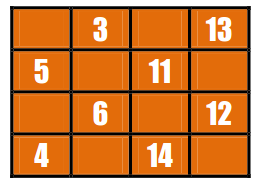
\includegraphics[width=.4\linewidth]{images/quadrado.png}
  \end{figure}

  Obs: Os números utilizados são de \textbf{1} a \textbf{16}.
\end{frame}

%------------------------------------------------

\begin{frame}{Problema 4 - Visão Espacial}
    Quantas caixas faltam para completar a pilha?

  \begin{figure}[htb!]
    \centering
    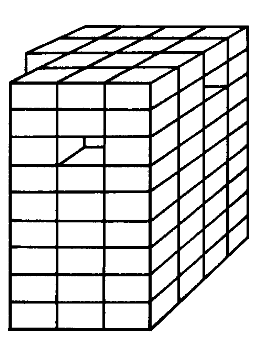
\includegraphics[width=.3\linewidth]{images/visao-espacial.png}
  \end{figure}

\end{frame}

%------------------------------------------------

\begin{frame}{Problema 5 - O castelo real}
    Uma cidade possui um castelo real. Para entrar no castelo é necessário
    um número secreto constituído por quatro algarismos. Sabe-se que:
    \begin{itemize}

        \item A soma dos quatro algarismos do número secreto é 9;
        \item Nenhum algarismo é zero;
        \item O número termina em 5;
        \item O número é maior que 2004.

    \end{itemize}

    Qual é o número secreto?
\end{frame}

%------------------------------------------------

\end{document}
